\documentclass[11pt]{standalone}
\usepackage{amssymb}
\usepackage{amsmath}
\usepackage[no-math]{fontspec}
\usepackage{unicode-math}
\usepackage{libertinus}
\usepackage{pgf,xcolor}
\usepackage{tikz}
\usetikzlibrary{arrows.meta, backgrounds}
\usepackage{pgfplots}
\pgfplotsset{compat=newest}

\definecolor{my_darkgray}{HTML}{484949}
\definecolor{my_lightgray}{HTML}{F3F4F4}
\definecolor{my_darkblue}{HTML}{005A94}
\definecolor{my_lightblue}{HTML}{CCDEE9}
\definecolor{my_yellow}{HTML}{FFEC7F}
\definecolor{my_red}{HTML}{E60000}
\definecolor{my_orange}{HTML}{E87846}

\begin{document}
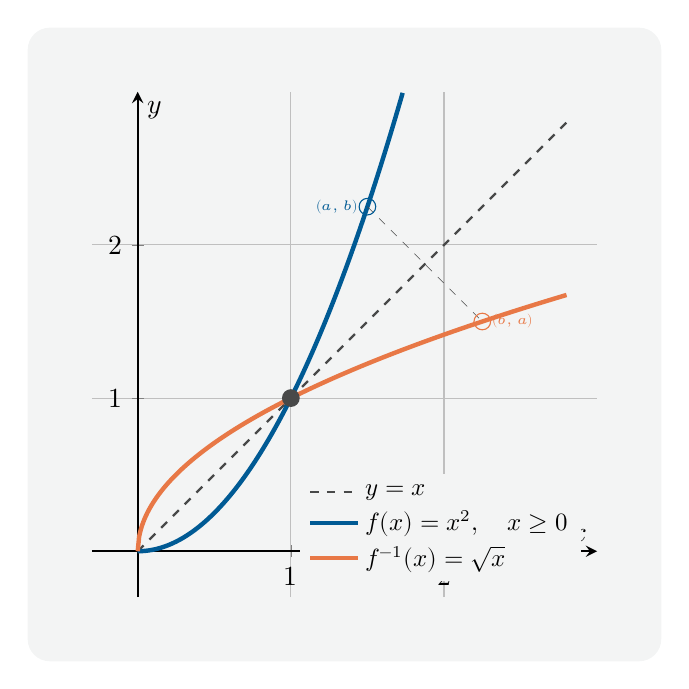
\begin{tikzpicture}[
    show background rectangle,
    background rectangle/.style={fill=my_lightgray, rounded corners=8pt},
    inner frame sep=0.8cm
]
\begin{axis}[
    axis lines=center,
    xlabel={$x$},
    ylabel={$y$},
    height=8cm, width=8cm,
    xmin=-0.3, xmax=3.0,
    ymin=-0.3, ymax=3.0,
    xtick={0,1,2},
    ytick={0,1,2},
    grid=both,
    axis equal,
    axis line style={thick},
    clip=false,
    legend style={
        font=\small,
        at={(0.97, 0.03)},
        anchor=south east,
        draw=none,
        fill=my_lightgray,
    },
    legend cell align=left,
]

% The line y=x (dashed, my_darkgray): the mirror axis
\addplot[draw=my_darkgray, dashed, thick, domain=0:2.8]{x};
\addlegendentry{$y = x$}

% f(x) = x^2 on domain [0, inf): the original function (my_darkblue)
% Restricted to [0, sqrt(3)] so f(x) stays within the plot window.
\addplot[draw=my_darkblue, samples=300, ultra thick, domain=0:1.73]
    {x^2};
\addlegendentry{$f(x)=x^2,\quad x \geq 0$}

% f^{-1}(x) = sqrt(x): the inverse function (my_orange)
% Defined for x in [0, inf); plotted for x in [0, 3].
\addplot[draw=my_orange, samples=300, ultra thick, domain=0:2.8]
    {sqrt(x)};
\addlegendentry{$f^{-1}(x)=\sqrt{x}$}

% Mark the fixed point (1,1), which lies on y=x and on both curves.
\addplot[only marks, mark=*, mark size=3pt,
         draw=my_darkgray, fill=my_darkgray]
    coordinates{(1, 1)};

% Example pair: the point (1.5, 2.25) on f and its reflection (2.25, 1.5) on f^{-1}.
% Thin dashed construction line connecting the pair through y=x.
\draw[dashed, my_darkgray, very thin]
    (axis cs:1.5, 2.25) -- (axis cs:2.25, 1.5);

\addplot[only marks, mark=o, mark size=3pt,
         draw=my_darkblue, fill=my_lightblue]
    coordinates{(1.5, 2.25)};
\node[left, font=\tiny, my_darkblue] at (axis cs:1.5, 2.25)
    {$(a,\,b)$};

\addplot[only marks, mark=o, mark size=3pt,
         draw=my_orange, fill=my_lightblue]
    coordinates{(2.25, 1.5)};
\node[right, font=\tiny, my_orange] at (axis cs:2.25, 1.5)
    {$(b,\,a)$};

\end{axis}
\end{tikzpicture}
\end{document}
